\chapter{Reduction from \PLCP to \EOPL}
\label{sec:PLCPtoEOPL}

In this section we present a polynomial-time reduction from the P-matrix Linear
Complementarity Problem (\PLCP) to \EOPL.
A Linear Complementarity Problem (LCP) is defined as follows. Now on by $[n]$ we mean set $\{1,\dots,n\}$.

\begin{definition}[LCP]
\label{def:lcp}
Given a matrix $M \in R^{d \times d}$ and a vector $\qq\in \Real^{d\times 1}$,
find a vector~{$\yy\in \Real^{d \times 1}$} such that:
\begin{equation}\label{eq:lcp}
M\yy\le \qq;\ \ \ \ \yy\ge 0;\ \ \ \ y_i(\qq - M\yy)_i =0,\ \forall i \in [n].
\end{equation}
\end{definition}
%
In general, an LCP may have no solution, and deciding whether one does is
\NP-complete~\cite{chung1989np}. If the matrix $M$ is a P-matrix, as defined
next, then the LCP $(M,\qq)$ has a unique solution for all $\qq\in \Real^{d\times
1}$.
%
\begin{definition}[P-matrix]
\label{def:Pmatrix}
A matrix $M \in \Real^{d \times d}$ is called a P-matrix if every principle
minor of $M$ is positive, {\em i.e.,} for every subset $S\subseteq[d]$, the
sub-matrix $N=[M_{i,j}]_{i\in S, j\in S}$ has strictly positive determinant. 
\end{definition}
%
In order to define a problem that takes all matrices $M$ as input without 
a promise, Megiddo~\cite{megiddo1988note} defined \PLCP as the following problem
(see also~\cite{megiddo1991total}).
%
\begin{definition}[\PLCP] \label{def:plcp} Given a matrix $M\in \Real^{d\times
d}$ and a vector $\qq\in \Real^{d\times 1}$, either:
\begin{enumerate}[label=(Q\arabic*)] \item Find vector $\yy \in \Real^{n
			\times 1}$ that satisfies (\ref{eq:lcp}) \item Produce a witness
that $M$ is a not a P-matrix, {\em i.e.,} find $S\subset [d]$ such that for
submatrix $N=[M_{i,j}]_{i\in S, j\in S}$, $det(N)\le 0$.  \end{enumerate}
\end{definition}
%
Later, Papadimitriou showed that \PLCP is in
\PPAD~\cite{papadimitriou1994complexity}, and then Daskalakis and Papadimitrou
showed that it is in \CLS~\cite{daskalakis2011continuous} (based on the
potential reduction method in~\cite{kojima1992interior}).  Designing a
polynomial-time solution for the \PLCP problem has been open for decades, at
least since the 1978 paper of Murty~\cite{murty1978computational} that provided
exponential-time examples for \emph{complementary pivoting algorithms}, such as 
\emph{Lemke's algorithm}~\cite{lemke1965bimatrix}, for
P-matrix Linear Complementarity Problems. Murty's family of P-matrices were
based on the Klee-Minty's cubes that had been used to give exponential-time
examples for the simplex method, and which inspired the research that led to
polynomial-time algorithms for Linear Programming. No similar polynomial-time
algorithms are known for \PLCP though.

Lemke's algorithm introduces an extra variable, say $z$, to the LCP polytope,
and follows a path on the $1$-skeleton of the new polytope (like the simplex 
method for linear programming) based
on complementary pivot rule (details below).  A general LCP need not have a
solution, and thus Lemke's algorithm is not guaranteed to terminate with a
solution.  However, for P-matrix LCPs, Lemke's algorithm terminates.  Indeed, if
Lemke's algorithm does not terminate with a solution, it provides a witness that
the matrix $M$ is not a P-matrix.  The structure of the path traced by Lemke's
algorithm is crucial for our reduction, so let us first briefly describe the
algorithm.

\subsection{Lemke's Algorithm}
\label{sec:lemke}

The explanation of Lemke's algorithm in this section is taken from \cite{GMSV}.
The problem is interesting only when $\qq \not \geq 0$, since otherwise $\yy = 0$ is a trivial solution. Let us introduce
slack variables $\ps$ to obtain the following equivalent formulation:
\begin{equation} \label{eq:b} \MM \yy  + \ps = \pq, \ \ \ \  \yy \geq 0, \ \ \ \ \ps \geq 0 \ \ \ \ \mbox{and} \ \ \ \ y_is_i = 0,\ \forall i\in[d].  \end{equation}

Let $\CQ$ be the polyhedron in $2d$ dimensional space defined by the first three conditions; we will assume that $\CQ$ is
non-degenerate (just for simplicity of exposition; this will not matter for our reduction).  
Under this condition, any solution to (\ref{eq:b}) will be a vertex of $\CQ$, since it must satisfy $2d$
equalities. Note that the set of solutions may be disconnected.
%
An ingenious idea of Lemke was to introduce a new variable and consider the system:
\begin{equation} \label{eq:c} \MM \yy  + \ps -z \one  = \pq, \ \ \ \  \yy \geq 0, \ \ \ \ \ps \geq 0, \ \ \ \  z \geq 0  \ \
\ \ \mbox{and} \ \ \ \ y_is_i = 0,\ \forall i\in[d].  \end{equation}
The next lemma follows by construction of (\ref{eq:c}).
\begin{lemma}\label{lem:lemke1}
Given $(\MM,\qq)$, $(\yy,\ps,z)$ satisfies \eqref{eq:c} with $z=0$ iff $\yy$ satisfies~\eqref{eq:lcp}.
\end{lemma}
%
Let $\CPol$ be the polyhedron in $2d + 1$ dimensional space defined by the first four conditions of \eqref{eq:c}, i.e.,
\begin{equation}\label{eq:cp}
\CPol = \{ (\yy,\ps, z) \ |\ \MM \yy  + \ps -z \one  = \pq, \ \ \ \yy \geq 0, \ \ \ \ps \geq 0, \ \ \  z \geq 0\};
\end{equation}
we will assume that $\CPol$ is {\em non-degenerate}.  

Since any solution to (\ref{eq:c}) must still satisfy $2d$ equalities in $\CPol$, the set of solutions, say
$S$, will be a subset of the one-skeleton of $\CPol$, i.e., it will consist of edges and vertices of $\CPol$.  Any solution to
the original system (\ref{eq:b}) must satisfy the additional condition $z = 0$ and hence will be a vertex of $\CPol$.



Now $S$ turns out to have some nice properties. Any point of $S$ is {\em fully labeled} in the sense that for each $i$, $y_i
= 0$ or $s_i = 0$.  We will say that a point of $S$ {\em has duplicate label i} if $y_i = 0$ and $s_i = 0$ are both satisfied
at this point. Clearly, such a point will be a vertex of $\CPol$ and it will have only one duplicate label.  Since there are
exactly two ways of relaxing this duplicate label, this vertex must have exactly two edges of $S$ incident at it.  Clearly, a
solution to the original system (i.e., satisfying $z = 0$) will be a vertex of $\CPol$ that does not have a duplicate label.  On
relaxing $z=0$, we get the unique edge of $S$ incident at this vertex.

As a result of these observations, we can conclude that $S$ consists of paths and cycles.  Of these paths, Lemke's algorithm
explores a special one.  An unbounded edge of $S$ such that the vertex of $\CPol$ it is incident on has $z > 0$ is called a
{\em ray}.  Among the rays, one is special -- the one on which $\yy = 0$. This is called the {\em primary ray} and the rest
are called {\em secondary rays}. Now Lemke's algorithm explores, via pivoting, the path starting with the primary ray. This
path must end either in a vertex satisfying $z = 0$, i.e., a solution to the original system, or a secondary ray. In the
latter case, the algorithm is unsuccessful in finding a solution to the original system; in particular, the original system
may not have a solution.  
We give the full pseudo-code for Lemke's algorithm in Appendix~\ref{app:lemke}.

%\noindent{\bf Remark:}  Observe that $z \one$ can be replaced by $z \pa$, where vector $\pa$ has a 1 in each row in which
%$\pq$ is negative and has either a 0 or a 1 in the remaining rows, without changing its role; in our algorithm, we will set
%a row of $\pa$ to 1 if and only if the corresponding row of $\pq$ is negative.  As mentioned above, if $\pq$ has no negative
%components, (\ref{eq:lcp}) has the trivial solution $\yy = 0$. Additionally, in this case Lemke's algorithm cannot be used for
%finding a non-trivial solution, since it is simply not applicable. 


%for the PLCP instance from a soluNote that these are the main two aspects of the End of Potential Line problem, however a number of details need to be taken care of, like binary representation of vertices, handling dummy solutions, potential representation, etc. Next we provide polynomial time reduction from PLCP to EoPL such that from a solution of the reduced instance, solution of the PLCP instance can be computed in polynomial time.

\subsection{Polynomial time reduction from \PLCP to \EOPL}

It is well known that if matrix $M$ is a P-matrix (\PLCP), then $z$ strictly
decreases on the path traced by Lemke's algorithm \cite{cottle2009linear}.
%; see Section \ref{subsec:Lemke} for a brief description of Lemke's algorithm. 
Furthermore, by a result of Todd~\cite[Section 5]{todd1976orientation}, paths traced by
complementary pivot rule can be locally oriented.  Based on these two facts, 
we now derive a polynomial-time reduction from \PLCP to \EOPL.

Let $\CI=(M,\qq)$ be a given \PLCP instance, and let $\CL$ be the length of the 
bit representation of $M$ and $\qq$. 
We will reduce $\CI$ to an \EOPL instance $\CE$ in time $poly(\CL)$. 
According to Definition~\ref{def:EOPL}, the instance $\CE$ is defined 
by its vertex set $\vert$, and procedures $S$ (successor), $P$ (predecessor) and $\pot$ (potential). 
Next we define each of these. 

As discussed in Section \ref{sec:lemke} the linear constraints of (\ref{eq:c})
on which Lemke's algorithm operates forms a polyhedron $\CPol$ given in
(\ref{eq:cp}). We assume that $\CPol$ is non-degenerate. This is without
loss of generality since, a typical way to ensure this is by perturbing $\qq$ so
that configurations of solution vertices remain unchanged
\cite{cottle2009linear}, and since $M$ is unchanged the LCP is still \PLCP. 
%A typical way to handle degenerate polyhedra is to purturbe $\qq$ such that its vertex configurations essentially remain unchanged, and therefore solution of the original problem can be retrived \cite{}. %, we call it $\CPol$. 

Lemke's algorithm traces a path on feasible points of (\ref{eq:c}) which is on
$1$-skeleton of $\CPol$ starting at $(\yy^0,\ps^0,z^0)$, where:
\begin{equation}\label{eq:v0}
\yy^0=0,\ \ \ \ \ z^0= |\min_{i \in [d]} q_i|,\ \ \ \ \  \ps^0=\qq+z\ones
\end{equation}
We want to capture
vertex solutions of (\ref{eq:c}) as vertices in \EOPL instance $\CE$. To
differentiate we will sometimes call the latter {\em configurations}. Vertex
solutions of (\ref{eq:c}) are exactly the vertices of polyhedron $\CPol$ with
either $y_i=0$ or $s_i=0$ for each $i\in [d]$. Vertices of (\ref{eq:c}) with
$z=0$ are our final solutions (Lemma \ref{lem:lemke1}). While each of its {\em
non-solution} vertex has a duplicate label. Thus, a vertex of this path can be
uniquely identified by which of $y_i=0$ and $s_i=0$ hold for each $i$ and its
duplicate label. This gives us a representation for vertices in the \EOPL
instance $\CE$. 

%Construct an EoPL instance as follows.
\medskip


\noindent{\bf \EOPL Instance $\CE$.}
\begin{itemize}
\item Vertex set $\vert=\{0,1\}^n$ where $n = 2d$. 
\item Procedures $S$ and $P$ as defined in Tables \ref{tab:S} and \ref{tab:P} respectively
\item Potential function $\pot:\vert \rightarrow \{0,1,\dots, 2^m-1\}$ defined in Table \ref{tab:F} for $m=\lceil ln(2\Delta^3)\rceil$, 
	  where $$\Delta=(n! \cdot I_{max}^{2d+1})+1$$ 
	  and $I_{max} = \max\{\max_{i,j\in [d]} M(i,j),\ \max_{i\in [d]} |q_i|\}$. 
\end{itemize}

For any vertex $\uu\in \vert$, the first $d$ bits of $\uu$ represent
which of the two inequalities, namely $y_i\ge 0$ and $s_i\ge 0$, are tight for
each $i \in [d]$. A valid setting of the second set of $d$ bits will have 
at most one non-zero bit -- if none is one then $z=0$, otherwise the location of one bit indicates the duplicate label. 
Thus, there are many invalid configurations, namely
those with more than one non-zero bit in the second set of $d$ bits. 
These are dummies that we will handle separately, and we define a procedure 
$\isvalid$ to identify non-dummy vertices in Table \ref{tab:iv} (in Appendix \ref{app:proc}). 
To go between ``valid'' vertices of $\CE$ and corresponding vertices of the Lemke polytope
$\CPol$ of LCP $\CI$, we define procedures $\eti$ and $\ite$ in Table
\ref{tab:ei} (in Appendix \ref{app:proc}).  
By construction of $\isvalid$, $\eti$ and $\ite$, the next lemma follows.
All the missing proofs of this section may be found in Appendix \ref{app:PLCPtoEOPL}.

\begin{lemma}\label{lem:vert}
If $\isvalid(\uu)=1$ then $\uu=\ite(\eti(\uu))$, and the corresponding vertex $(\yy,\ps,z)\in \eti(\uu)$ of $\CPol$ is feasible in (\ref{eq:c}). If $(\yy,\ps,z)$ is a feasible vertex of (\ref{eq:c}) then $\uu=\ite(\yy,\ps,z)$ is a valid configuration, {\em i.e.,} $\isvalid(\uu)=1$.
\end{lemma}
%\begin{proof}
%The only thing that can go wrong is that the matrix $A$ generated in $\isvalid$ and $\eti$ procedures are singular, or the set of double lables $DL$ generated in $\ite$ has more than one elements. 
%Each of these are possible only when more than $2d+1$ equalities of $\CPol$ hold at the corresponding point $(\yy,\ps,z)$, violating non-degeneracy assumption. 
%\end{proof}

\begin{figure}[htbp]
   \centering
\vspace{-1cm}

  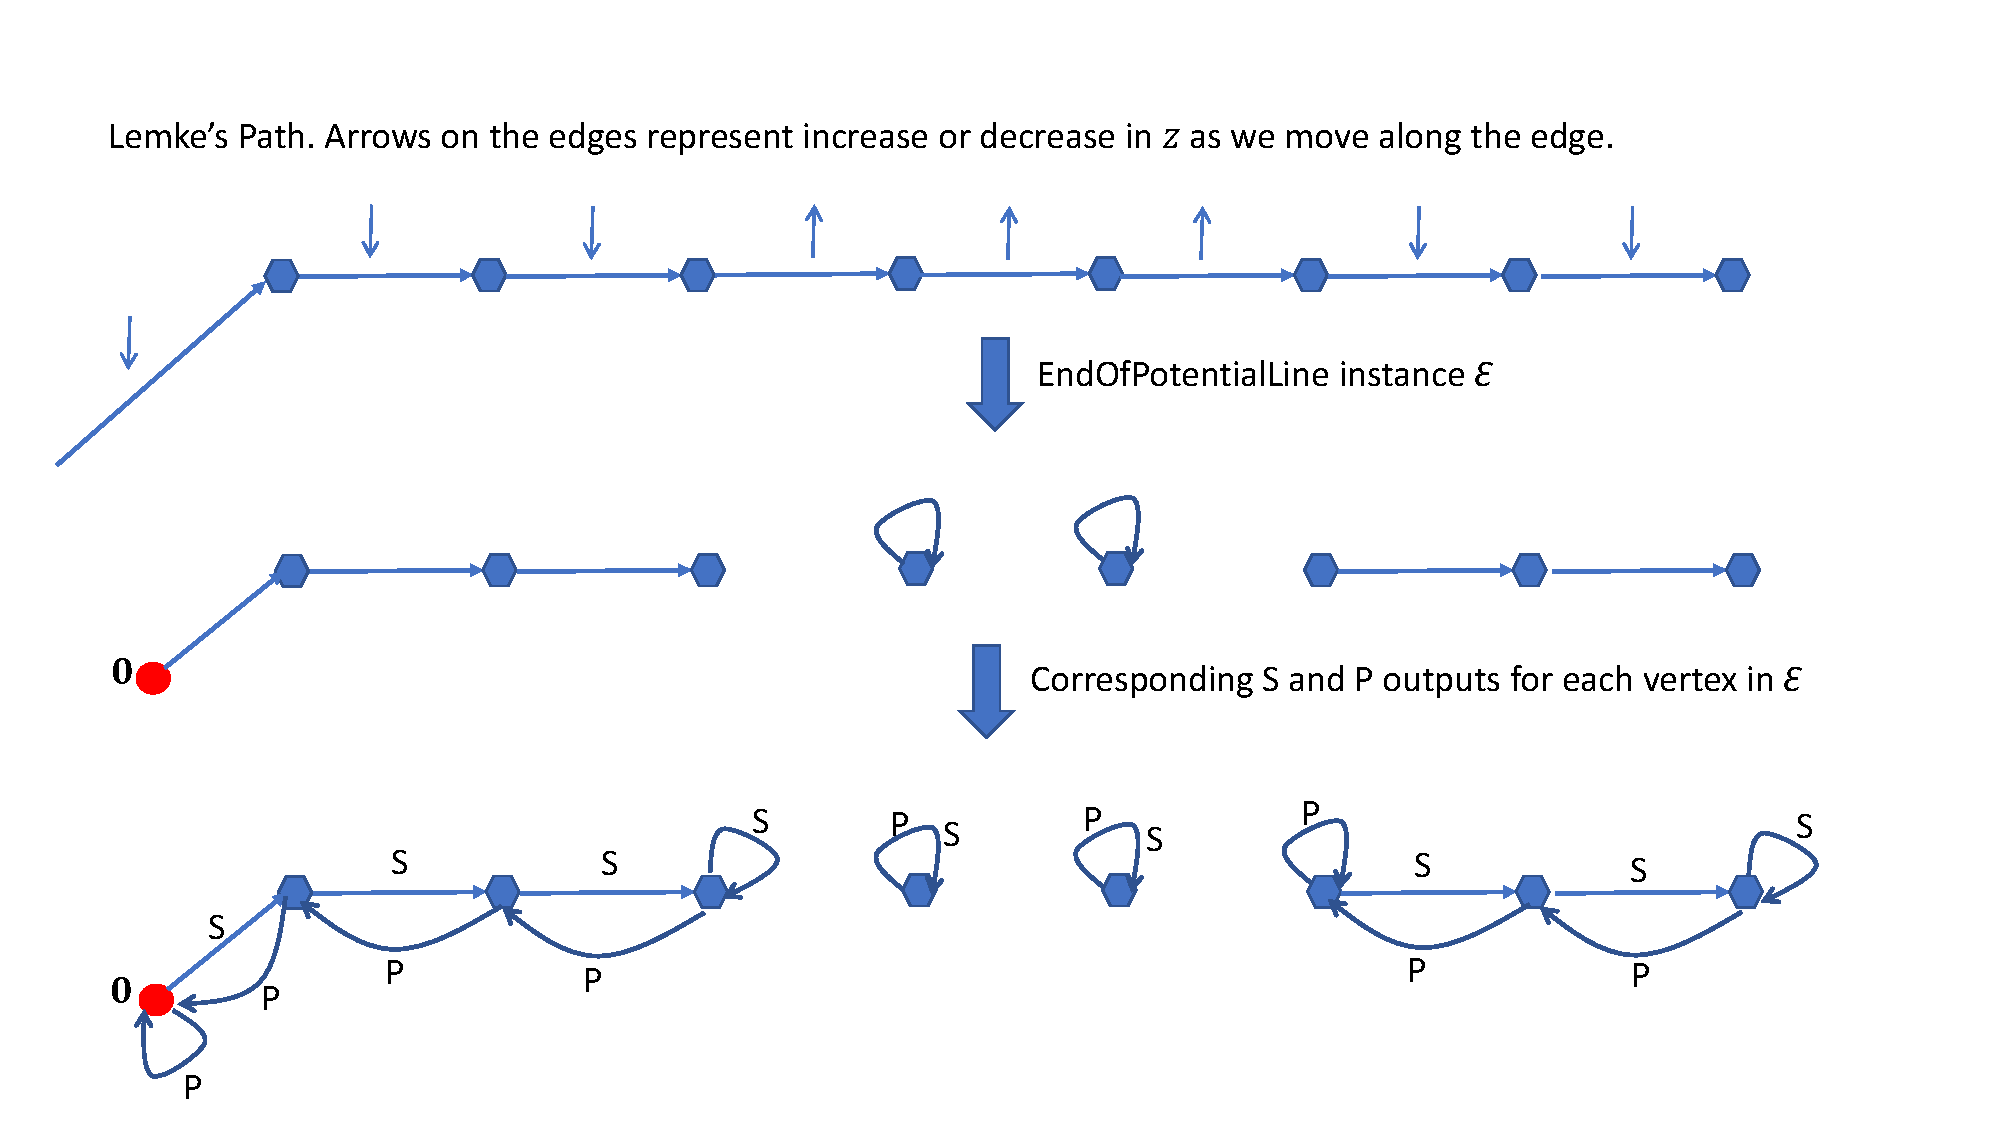
\includegraphics[width=\textwidth]{plcp-fig.pdf}
 \caption{Construction of $S$ and $P$ for \EOPL instance $\CE$ from the Lemke
 	path. The first path is the Lemke path and the arrows on its edges indicate
 	whether the value of $z$ increases or decreases along the edge.  Note that
 	the end or start of a path in $\CE$, which is an intermediate vertex in
 	Lemke path that has either decreased and then increased, or increased and then
 	decreased in the value of $z$, is a violation of $M$ being a $P$ matrix
 	\cite{cottle2009linear}, i.e., $\PLt$ type solution of
 	\PLCP.}
 	\label{fig:path}
\end{figure}   


The main idea behind procedures $S$ and $P$, given in Tables \ref{tab:S} and
\ref{tab:P} respectively, is the following (also see Figure \ref{fig:path}):
Make dummy configurations in $\vert$ point to themselves with cycles of
length one, so that they can never be solutions. 
The starting vertex $0^n \in \vert$ points to the configuration that corresponds
to the first vertex of the Lemke path, namely $\uu^0=\ite(\yy^0,\ps^0,z^0)$. 
Precisely, $S(0^n)=\uu^0$, $P(\uu^0)=0^n$ and $P(0^n)=0^n$ (start of
a path). 

For the remaining cases, let $\uu\in \vert$ have corresponding representation
$\xx=(\yy,\ps,z)\in \CPol$, and suppose $\xx$ has a duplicate label. As one
traverses a Lemke path for a P-LCPs, the value of $z$ monotonically decreases.
So, for $S(\uu)$ we compute the adjacent vertex $\xx'=(\yy',\ps',z')$ of $\xx$
on Lemke path such that the edge goes from $\xx$ to $\xx'$, and if the $z'<z$,
as expected, then we point $S(\uu)$ to configuration of $\xx'$ namely
$\ite(\xx')$. Otherwise, we let $S(\uu)=\uu$. Similarly, for $P(\uu)$, we find
$\xx'$ such that edge is from $\xx'$ to $\xx$, and then we let $P(\uu)$ be
$\ite(\xx')$ if $z'>z$ as expected, otherwise $P(\uu)=\uu$. 

For the case when $\xx$ does not have a duplicate label, then we have $z=0$. This is
handled separately since such a vertex has exactly one incident edge on the Lemke
path, namely the one obtained by relaxing $z=0$. According to the direction of 
this edge, we do similar process as before. For example, if the edge goes from 
$\xx$ to $\xx'$, then, if $z'<z$, we set $S(\uu)=\ite(\xx')$ else $S(\uu)=\uu$,
and we always set $P(\uu)=\uu$.  In case the edge goes from $\xx'$ to $\xx$, we
always set $S(\uu)=\uu$, and we set $P(\uu)$ depending on whether or not $z'>z$.

%If $\xx$ is a solution of the original LCP, i.e., $z=0$, then exactly one of $S(\uu)$ or $P(\uu)$ would point to the configuration of the vertex obtained by relaxing $z=0$ at $xx$, while the other will point back to $\uu$ itself. Which one of the two cases happen depends on what orientation corresponding edge on Lemke's path has. 
%
%For the rest, if $l$ is the duplicate label at $\xx$ then let $\xx^1$ and $\xx^2$ be the two vertices obtained by relaxing $y_l=0$ and $s_l=0$ at $\xx$. Lemke's algoithm must have traversed either $\xx^1$ to $\xx$ to $\xx^2$, or $\xx^2$ to $\xx$ to $\xx^1$. Which of the two would tell us output of $S(\uu)$ and $P(\uu)$. Todd \cite{} gives a polynomial time procedure to find out which one is the case based on signs of certain determinants of matrices formed using the sets of non-zero and zero variables at these three vertices, and $(M,\qq)$. Based on this we output either representation of $\xx^1$ or $\xx^2$. 
\medskip

The potential function $\pot$, formally defined in Table \ref{tab:F},
gives a value of zero to dummy vertices and the starting vertex $0^n$. To all
other vertices, essentially it is $((z^0-z) * \Delta^2)+1$. Since value of $z$
starts at $z^0$ and keeps decreasing on the Lemke path this value will keep
increasing starting from zero at the starting vertex $0^n$. Multiplication by
$\Delta^2$ will ensure that if $z_1>z_2$ then the corresponding potential values 
will differ by at least one. This is because, since $z_1$ and $z_2$ are 
coordinates of two vertices of polytope $\CPol$, their maximum value is $\Delta$
and their denominator is also bounded above by $\Delta$. Hence $z_1-z_2\le
1/\Delta^2$ (Lemma \ref{lem:pot}).  
% REWRITE
%Thus, if after change of scales $1/2*\Delta^2$ defines a unit then
%corresponding integers will differ by at least one. 

To show correctness of the reduction we need to show two things: $(i)$ All the procedures are well-defined and polynomial time. $(ii)$ We can construct a solution of $\CI$ from a solution of $\CE$ in polynomial time. 



\begin{table}
\begin{minipage}{0.73\textwidth}
\caption{Successor Procedure $S(\uu)$}\label{tab:S}
\begin{tabular}{|l|}
\hline
%$S(\uu)$\\
%\small{
\hspace{0pt}{\bf If} $\isvalid(\uu)=0$ {\bf then} {\bf Return} $\uu$\\
\hspace{0pt}{\bf If} $\uu=0^n$ {\bf then} {\bf Return} $\ite(\yy^0,\ps^0,z^0)$\\
\hspace{0pt}$\xx=(\yy,\ps,z) \leftarrow \eti(\uu)$\\
%\hspace{5pt} {\bf If} $z=0$ {\bf then} {\bf Return} $\uu$
\hspace{0pt}{\bf If} $z=0$ {\bf then} \\
\hspace{5pt} $\xx^1\leftarrow$ vertex obtained by relaxing $z=0$ at $\xx$ in $\CPol$. \\
\hspace{5pt} {\bf If} Todd \cite{todd1976orientation} prescribes edge from $\xx$ to $\xx^1$ \\
\hspace{10pt} {\bf then} set $\xx'\leftarrow \xx^1$. {\bf Else Return} $\uu$ \\
\hspace{0pt}{\bf Else} set $l\leftarrow $ duplicate label at $\xx$\\
%\hspace{5pt} $(\yy',\ps',z') \leftarrow$ Next vertex from $(\yy,\ps,z)$ in $\CPol$ as preѕcribed by Todd \cite{todd}. 
\hspace{5pt} $\xx^1\leftarrow $ vertex obtained by relaxing $y_l=0$ at $\xx$ in $\CPol$ \\
\hspace{5pt} $\xx^2\leftarrow $ vertex obtained by relaxing $s_l=0$ at $\xx$ in $\CPol$ \\
\hspace{5pt} {\bf If} Todd \cite{todd1976orientation} prescribes edge from $\xx$ to $\xx^1$ \\
\hspace{10pt} {\bf then} $\xx'=\xx^1$ \\
\hspace{5pt} {\bf Else} $\xx'=\xx^2$\\
\hspace{0pt}Let $\xx'$ be $(\yy',\ps',z')$. \\
\hspace{0pt}{\bf If} $z>z'$ {\bf then} {\bf Return} $\ite(\xx')$. {\bf Else} {\bf Return} $\uu$.\\
%\hspace{5pt} {\bf Return} $\ite(\xx')$.
%}
\hline
\end{tabular}
\end{minipage}%
\hspace{-1cm}
\begin{minipage}{0.23\textwidth}
\caption{Potential Value $\pot(\uu)$}\label{tab:F}
\begin{tabular}{|l|}
\hline
%\small{
%$\pot(\uu)$\\
\hspace{0pt} {\bf If} $\isvalid(\uu)=0$ \\
\hspace{5pt} {\bf then} {\bf Return} $0$\\
\hspace{0pt} {\bf If} $\uu=0^n$\\
\hspace{5pt}  {\bf then} {\bf Return} $0$\\
\hspace{0pt} $(\yy,\ps,z) \leftarrow \eti(\uu)$\\
\hspace{0pt} {\bf Return} $\lfloor \Delta^2*(\Delta -z)\rfloor$\\
%}
\hline
\end{tabular}
\end{minipage}
\end{table}



\begin{table}[!htb]
\caption{Predecessor Procedure $P(\uu)$}\label{tab:P}
\begin{tabular}{|l|}
\hline
%$P(\uu)$\\
%\small{
\hspace{0pt} {\bf If} $\isvalid(\uu)=0$ {\bf then} {\bf Return} $\uu$\\
\hspace{0pt} {\bf If} $\uu=0^n$ {\bf then} {\bf Return} $\uu$\\
\hspace{0pt} $(\yy,\ps,z) \leftarrow \eti(\uu)$\\
\hspace{0pt} {\bf If} $(\yy,\ps,z)=(\yy^0,\ps^0,z^0)$ {\bf then} {\bf Return} $0^n$\\
%\hspace{5pt} $l\leftarrow $ duplicate label at $(\yy,\ps,z)$, $(\yy',\ps',z') \leftarrow $ $Prev(\vv,l)$.\\
%\hspace{5pt} $(\yy',\ps',z') \leftarrow$ Previous vertex from $(\yy,\ps,z)$ in $\CPol$ as preѕcribed by Todd \cite{todd}. \\
\hspace{0pt} {\bf If} $z=0$ {\bf then} \\
\hspace{5pt} $\xx^1\leftarrow$ vertex obtained by relaxing $z=0$ at $\xx$ in $\CPol$. \\
\hspace{5pt} {\bf If} Todd \cite{todd1976orientation} prescribes edge from $\xx^1$ to $\xx$ {\bf then} set $\xx'\leftarrow \xx^1$. {\bf Else Return} $\uu$\\
\hspace{0pt} {\bf Else}\\
\hspace{5pt} $l\leftarrow $ duplicate label at $\xx$\\
\hspace{5pt} $\xx^1\leftarrow $ vertex obtained by relaxing $y_l=0$ at $\xx$ in $\CPol$ \\
\hspace{5pt} $\xx^2\leftarrow $ vertex obtained by relaxing $s_l=0$ at $\xx$ in $\CPol$ \\
\hspace{5pt} {\bf If} Todd \cite{todd1976orientation} prescribes edge from $\xx^1$ to $\xx$ {\bf then} $\xx'=\xx^1$ {\bf Else} $\xx'=\xx^2$\\
\hspace{0pt} Let $\xx'$ be $(\yy',\ps',z')$. {\bf If} $z<z'$ {\bf then} {\bf Return} $\ite(\xx')$. {\bf Else} {\bf Return} $\uu$.\\
%\hspace{5pt} {\bf Return} $\ite(\xx')$.
%}
\hline
\end{tabular}
\end{table}



\begin{lemma}\label{lem:PSF}
Functions $P$, $S$ and $\pot$ of instance $\CE$ are well defined, making $\CE$ a valid \EOPL instance. 
\end{lemma}
%\begin{proof}
%Since all the three procedures are polynomial time in $\CL$, they can be defined
%	by $poly(\CL)$ sized Boolean circuits. Furthermore, for any $\uu \in \vert$,
%	$S(\uu),P(\uu) \in \vert$. For $\pot$, since value of $z \in [0,\ \Delta-1]$ we
%	have $0\le \Delta^2(\Delta-z)\le \Delta^3$. Therefore, $\pot(\uu)$ is an
%	integer that is at most $2*\Delta^3$ and hence is in set $\{0,\dots, 2^m-1\}$. 
%\end{proof}

There are two possible types of solutions of an \EOPL instance. One indicates
the beginning or end of a line, and the other is a vertex with locally optimal
potential (that does not point to itself). 
First we show that the latter case never arise. For this, we need the
next lemma, which shows that potential differences in two adjacent
configurations adheres to differences in the value of $z$ at corresponding
vertices.

\begin{lemma}\label{lem:pot}
Let $\uu \neq \uu'$ be two valid configurations, i.e.,
	$\isvalid(\uu)=\isvalid(\uu')=1$, and let $(\yy,\ps,z)$ and $(\yy',\ps',z')$
	be the corresponding vertices in $\CPol$. Then the following holds: $(i)$
	$\pot(\uu)=\pot(\uu')$ iff $z=z'$. $(ii)$ $\pot(\uu)>\pot(\uu')$ iff $z<z'$.
\end{lemma}
%\begin{proof}
%Among the valid configurations all except $0^n$ has positive $\pot$ value. Therefore, wlog let $\uu,\uu'\neq 0^n$. For these we have $\pot(\uu)=\lfloor \Delta^2*(\Delta -z)\rfloor$, and $\pot(\uu')=\lfloor \Delta^2*(\Delta -z')\rfloor$. 
%
%Note that since both $z$ and $z'$ are coordinates of vertices of $\CPol$, whose description has highest coefficient of $\max\{\max_{i,j\in [d]} M(i,j),\max_{i\in [d]} |q_i|\}$, and therefore their numerator and denominator both are bounded above by $\Delta$. Therefore, if $z< z'$ then 
%\[
%z'-z\ge \frac{1}{\Delta^2} \Rightarrow ((\Delta-z) - (\Delta - z'))*\Delta^2 \ge 1 \Rightarrow \pot(\uu)-\pot(\uu') \ge 1
%\]
%
%For $(i)$, if $z=z'$ then clearly $\pot(\uu)=\pot(\uu')$, and from the above argument it also follows that if $\pot(\uu)= \pot(\uu')$ then it can not be the case that $z\neq z'$. Similarly for $(ii)$, if $\pot(\uu)>\pot(\uu')$ then clearly, $z'>z$, and from the above argument it follows that if $z'>z$ then it can not be the case that $\pot(\uu')\ge \pot(\uu)$. 
%\end{proof}

Using the above lemma, we will next show that instance $\CE$ has no local maximizer. 

\begin{lemma}\label{lem:t}
Let $\uu,\vv \in \vert$ s.t. $\uu\neq \vv$, $\vv=S(\uu)$, and $\uu=P(\vv)$. Then $\pot(\uu)< \pot(\vv)$.
\end{lemma}
\begin{proof}
Let $\xx=(\yy,\ps,z)$ and $\xx'=(\yy',\ps',z')$ be the vertices in polyhedron $\CPol$ corresponding to $\uu$ and $\vv$ respectively. From the construction of $\vv=S(\uu)$ implies that $z'<z$. Therefore, using Lemma \ref{lem:pot} it follows that $\pot(\vv)<\pot(\uu)$.
%Both $\uu$ and $\vv$ can not be dummy configurations because otherwise they will point to themselves in $P$ and $S$ both. For the rest let $\xx=(\yy,\ps,z)$ and $\xx'=(\yy',\ps',z')$ be the vertices in polyhedron $\CPol$ corresponding to $\uu$ and $\vv$ respectively. Since these are not dummy, we have an edge from $\xx$ to $\xx'$. Further, using Lemma \ref{lem:pot} it must be the case that $z<z'$. In otherwords, if $\sigma=\xx'-\xx$ then $\simga(z)>0$. This contradicts $M$ being a P-matrix, and the submatrix corresponding non-zero gives a witness. 
\end{proof}

Due to Lemma \ref{lem:t} the only type of solutions available in $\CE$ is where $S(P(\uu))\neq \uu$ and $P(S(\uu))\neq \uu$. Next two lemmas shows how to construct solutions of $\CI$ from these. 

\begin{lemma}\label{lem:t1}
Let $\uu \in \vert$, $\uu \neq 0^n$. % be such that $\isvalid(\uu)=1$, and let $(\yy,\ps,z)=\eti(\uu)$. 
If $P(S(\uu))\neq \uu$ or $S(P(\uu))\neq \uu$, then $\isvalid(\uu)=1$, and for $(\yy,\ps,z)=\eti(\uu)$ if $z=0$ then $\yy$ is a $\PLo$ type solution of \PLCP instance $\CI=(M,\qq)$. 
\end{lemma}
\begin{proof}
By construction, if $\isvalid(\uu) = 0$, then $S(P(\uu))=\uu$ and $P(S(\uu))=\uu$, therefore $\isvalid(\uu)=0$ when $\uu$ has a predecessor or successor different from $\uu$.
Given this, from Lemma \ref{lem:vert} we know that $(\yy,\ps,z)$ is a feasible vertex in (\ref{eq:c}). Therefore, if $z=0$ then using Lemma \ref{lem:lemke1} we have a solution of the LCP (\ref{eq:lcp}), {\em i.e.,} a type $\PLo$ solution of our \PLCP instance $\CI=(\MM,\qq)$.
%
%If it has a duplicate label, then it has two incident edges say from vertices $\xx'$ and $\xx''$. Let the corresponding configurations in $\CE$ be $\uu'$ and $\uu''$ respectively. Due to Lemma \ref{lem:vert}, we can consistently go between $\uu$'s and $\xx$'s using $\ite$ and $\eti$ procedues. Further, if $\uu'=S(\uu)$ then when we apply $P$ to $\uu'$ we will get back $\uu$, due to the property of Lemke's algorithm and cannonical orientation obtained by Todd \cite{todd}. Similarly, if $\uu''=P(\uu)$ then $S(\uu'')$ will give $\uu$ back. Therefore, $\uu$ can not be a vertex with duplicate label.
%
%The only remaining valid configurations correspond to vertices of $\CPol$ that satisfy $y_is_i=0,\ \forall i \in[d]$, and $z=0$. Since solutions of (\ref{eq:c}) are exactly the solutions of (\ref{eq:lcp}) (Lemma \ref{lem:lemke1}) we get $\PLo$ type solution of our given PLCP instance $\CI=(M,\qq)$.
\end{proof}

\begin{lemma}\label{lem:t2}
Let $\uu \in \vert$, $\uu \neq 0^n$ such that $P(S(\uu))\neq \uu$ or $S(P(\uu))\neq \uu$, and let $\xx=(\yy,\ps,z)=\eti(\uu)$. 
If $z\neq 0$ then $\xx$ has a duplicate label, say $l$. And for directions $\sigma_1$ and $\sigma_2$ obtained by relaxing $y_l=0$ and $s_l=0$ respectively at $\xx$, we have $\sigma_1(z)*\sigma_2(z)\ge 0$, where $\sigma_i(z)$ is the coordinate corresponding to $z$. 
\end{lemma}
\begin{proof}
From Lemma \ref{lem:t1} we know that $\isvalid(\uu)=1$, and therefore from Lemma \ref{lem:vert}, $\xx$ is a feasible vertex in (\ref{eq:c}).
From the last line of Tables \ref{tab:S} and \ref{tab:P} observe that $S(\uu)$ points to the configuration of vertex next to $\xx$ on Lemke's path only if it has lower $z$ value otherwise it gives back $\uu$, and similarly $P(\uu)$ points to the previous only if value of $z$ increases.

%For both the cases we have that either $S(\uu)\neq \uu$ or $P(\uu)\neq \uu$. 
%}

First consider the case when $P(S(\uu))\neq \uu$. Let $\vv=S(\uu)$ and corresponding vertex in $\CPol$ be $(\yy',\ps',z')=\eti(\vv)$. 
If $\vv\neq \uu$, then from the above observation we know that $z'>z$, and in that
case again by construction of $P$ we will have $P(\vv)=\uu$, contradicting
$P(S(\uu))\neq \uu$. Therefore, it must be the case that $\vv=\uu$.
Since $z\neq 0$ this happens only when the next vertex on Lemke path after $\xx$ has
higher value of $z$ (by above observation). As a consequence of $\vv=\uu$, we also have $P(\uu)\neq \uu$. By construction of $P$ this implies for 
$(\yy'',\ps'',z'')=\eti(P(\uu))$, $z''>z$. Putting both together we get 
increase in $z$ when we relax $y_l=0$ as well as when we relax $s_l=0$ at
$\xx$.

For the second case $S(P(\uu))\neq \uu$ similar argument gives that value of $z$ decreases when we relax $y_l=0$ as well as when we relax $s_l=0$ at
$\xx$. The proof follows.
\end{proof}

Finally, we are ready to prove our main result of this section using Lemmas
\ref{lem:t}, \ref{lem:t1} and \ref{lem:t2}. Together with Lemma \ref{lem:t2},
we will use the fact that on Lemke path $z$ monotonically decreases if $M$ is a
P-matrix or else we get a witness that $M$ is not a
P-matrix~\cite{cottle2009linear}. 
%Lemmas \ref{lem:t1} and \ref{lem:t2} gives the two possible types of solutions
%of the PLCP problem. That is either actual solution of the corresponding LCP
%instance, or a witness that the given matrix is not a $P$-matrix. Recall that
%checking the latter is co-NP-complete. Thus next theorem follows from Lemmas
%\ref{lem:PSF}, \ref{lem:t1} and \ref{lem:t2}.

\begin{theorem}
\PLCP reduces to \EOPL in polynomial-time. 
\end{theorem}
\begin{proof}
	Given an instance of $\CI=(\MM,\qq)$ of \PLCP, where $M\in \Real^{d\times d}$ and $\qq\in \Real^{d\times 1}$ reduce it to an instance $\CE$ of \EOPL as described above with vertex set $\vert=\{0,1\}^{2d}$ and procedures $S$, $P$ and $\pot$ as given in Table \ref{tab:S}, \ref{tab:P}, and \ref{tab:F} respectively.

Among solutions of \EOPL instance $\CE$, there is no local potential maximizer,
	i.e., $\uu\neq \vv$ such that $\vv=S(\uu)$, $\uu=P(\vv)$ and $\pot(\uu)>\pot(\vv)$
	due to Lemma \ref{lem:t}. We get a solution $\uu \neq 0$ such that either
	$S(P(\uu))\neq \uu$ or $P(S(\uu))\neq \uu$, then by Lemma \ref{lem:t1} it is
	valid configuration and has a corresponding vertex $\xx=(\yy,\ps,z)$ in
	$\CPol$. Again by Lemma~\ref{lem:t1} if $z=0$ then $\yy$ is a $\PLo$ type solution
	of our \PLCP instance $\CI$. On the other hand, if $z>0$ then from Lemma
	\ref{lem:t2} we get that on both the two adjacent edges to $\xx$ on Lemke
	path the value of $z$ either increases or deceases. This gives us a minor of $M$
	which is non-positive~\cite{cottle2009linear}, 
	i.e., a $\PLt$ type solution of the $\PLCP$	instance $\CI$.
\end{proof}

\newpage

%%%%%%%%%%%%%%%%%%%%
% END OF 12 pages!
%%%%%%%%%%%%%%%%%%%%


